\chapter{Results and Discussion}
\label{sec:chapterResults}

% ══════════════════════════════════════════════════════════════════════════
% REQUIRED PACKAGES (add to main .tex preamble if not already present):
%   \usepackage{pgfplots}
%   \pgfplotsset{compat=1.18}
%   \usepgfplotslibrary{groupplots}
%   \usepackage{booktabs}
%   \usepackage{xcolor}       % for \definecolor
%   \usepackage{multirow}     % for multi-row cells (optional)
% ══════════════════════════════════════════════════════════════════════════

% All tables and figures are generated from actual experimental data via
% generate_results.py. Discussion sections reference verified metric values.

% ── Consistent model colours for all figures ──
\definecolor{clrLGBM}{HTML}{1f77b4}
\definecolor{clrCB}{HTML}{d62728}
\definecolor{clrRF}{HTML}{2ca02c}
\definecolor{clrFT}{HTML}{ff7f0e}
\definecolor{clrLR}{HTML}{9467bd}
\definecolor{clrOCSVM}{HTML}{7f7f7f}

This chapter is organised in practical execution order:
each section corresponds to a well-defined experimental step whose artefacts (tables, figures, metrics JSON files) are produced by a specific code pipeline run.
All metrics are defined in Section~\ref{sec:metrics} of the Methodology chapter.

% ══════════════════════════════════════════════════════════════════════════
%  1 — BASELINE MODEL COMPARISON
% ══════════════════════════════════════════════════════════════════════════

\section{Baseline Model Comparison (No Imbalance Strategy)}
\label{sec:baseline_results}

This section compares all models tuned via Optuna TPE (50 trials,
5-fold stratified cross-validation, scoring\,=\,PR-AUC)
\emph{without} any imbalance handling strategy.
Results are reported on the holdout test set using the
$F_2$-maximising threshold~($\tau$) obtained from inner validation
(median across folds).
The same trained models and probability scores are later reused for
the threshold sensitivity analysis (Section~\ref{sec:threshold_sensitivity}),
where alternative threshold strategies are applied \emph{without retraining}.

% ─────────────────── ULB 2013 ───────────────────

\subsection{ULB Credit Card 2013}

\begin{table}[ht!]
\centering
\caption{Baseline comparison on ULB 2013 (strategy\,=\,None, threshold\,=\,max-$F_2$).}
\label{tab:baseline_ulb}
\begin{tabular}{l c c c c c c c c}
\toprule
Model & PR-AUC & ROC-AUC & $F_1$ & $F_2$ & Precision & Recall & $\tau$ & Brier \\
\midrule
LR         & 0.7419 & 0.9649 & 0.7489 & 0.7992 & 0.6777 & 0.8367 & 0.0435 & 0.00075 \\
RF         & 0.8667 & 0.9591 & 0.8309 & 0.8583 & 0.7890 & 0.8776 & 0.1920 & 0.00039 \\
LGBM       & 0.8744 & 0.9749 & 0.8235 & 0.8434 & 0.7925 & 0.8571 & 0.1038 & 0.00039 \\
CatBoost   & 0.8847 & 0.9776 & 0.8333 & 0.8534 & 0.8019 & 0.8673 & 0.0539 & 0.00034 \\
FT-Trans.  & 0.8562 & 0.9748 & 0.7545 & 0.8074 & 0.6803 & 0.8469 & 0.0350 & 0.00048 \\
OCSVM      & 0.3354 & 0.9534 & 0.4145 & 0.5268 & 0.3058 & 0.6429 & 2.4887 & 0.00832 \\
\bottomrule
\end{tabular}
\end{table}

\begin{table}[ht!]
\centering
\caption{Operational metrics on ULB 2013 (strategy\,=\,None, threshold\,=\,max-$F_2$).}
\label{tab:ops_ulb}
\begin{tabular}{l c c c c c}
\toprule
Model & Alert Rate & FP/TP & P@$k$ & R@$k$ & $k$ \\
\midrule
LR         & 0.00212 & 0.4756 & 0.3063 & 0.8878 & 284 \\
RF         & 0.00191 & 0.2674 & 0.3099 & 0.8980 & 284 \\
LGBM       & 0.00186 & 0.2619 & 0.3099 & 0.8980 & 284 \\
CatBoost   & 0.00186 & 0.2471 & 0.3099 & 0.8980 & 284 \\
FT-Trans.  & 0.00214 & 0.4699 & 0.3063 & 0.8878 & 284 \\
OCSVM      & 0.00362 & 2.2698 & 0.2430 & 0.7041 & 284 \\
\bottomrule
\end{tabular}
\end{table}

\begin{figure}[ht!]
  \centering
  
\includegraphics[width=0.78\textwidth]{figures/ulb/prauc_bar_baseline.pdf}
  \caption{PR-AUC for all models on ULB 2013 (baseline, Optuna, $F_2$ threshold).}
  \label{fig:prauc_ulb}
\end{figure}

% ─────────────────── BAF Base ───────────────────

\subsection{BAF Base}

\begin{table}[ht!]
\centering
\caption{Baseline comparison on BAF Base (strategy\,=\,None, threshold\,=\,max-$F_2$).}
\label{tab:baseline_baf}
\begin{tabular}{l c c c c c c c c}
\toprule
Model & PR-AUC & ROC-AUC & $F_1$ & $F_2$ & Precision & Recall & $\tau$ & Brier \\
\midrule
LR         & 0.1432 & 0.8745 & 0.1871 & 0.2868 & 0.1185 & 0.4447 & 0.0527 & 0.01009 \\
RF         & 0.1588 & 0.8778 & 0.2048 & 0.2941 & 0.1360 & 0.4148 & 0.0631 & 0.01007 \\
LGBM       & 0.1768 & 0.8985 & 0.2224 & 0.3159 & 0.1490 & 0.4388 & 0.0636 & 0.00986 \\
CatBoost   & 0.1796 & 0.8980 & 0.2106 & 0.3143 & 0.1359 & 0.4678 & 0.0573 & 0.00984 \\
FT-Trans.  & 0.1797 & 0.8974 & 0.2246 & 0.3160 & 0.1515 & 0.4338 & 0.0584 & 0.00986 \\
OCSVM      & 0.0190 & 0.6279 & 0.0449 & 0.0805 & 0.0258 & 0.1714 & -40.26 & 0.02061 \\
\bottomrule
\end{tabular}
\end{table}

\begin{table}[ht!]
\centering
\caption{Operational metrics on BAF Base (strategy\,=\,None, threshold\,=\,max-$F_2$).}
\label{tab:ops_baf}
\begin{tabular}{l c c c c c}
\toprule
Model & Alert Rate & FP/TP & P@$k$ & R@$k$ & $k$ \\
\midrule
LR         & 0.04140 & 7.4393 & 0.2720 & 0.1233 & 1000 \\
RF         & 0.03365 & 6.3552 & 0.3120 & 0.1414 & 1000 \\
LGBM       & 0.03249 & 5.7128 & 0.3420 & 0.1550 & 1000 \\
CatBoost   & 0.03798 & 6.3605 & 0.3420 & 0.1550 & 1000 \\
FT-Trans.  & 0.03158 & 5.5998 & 0.3360 & 0.1523 & 1000 \\
OCSVM      & 0.07321 & 37.7328 & 0.0300 & 0.0136 & 1000 \\
\bottomrule
\end{tabular}
\end{table}

\begin{figure}[ht!]
  \centering
  
\includegraphics[width=0.78\textwidth]{figures/baf/prauc_bar_baseline.pdf}
  \caption{PR-AUC for all models on BAF Base (baseline, Optuna, $F_2$ threshold).}
  \label{fig:prauc_baf}
\end{figure}

\paragraph{Discussion.}
  On ULB~2013, all supervised models achieve high PR-AUC values ($>0.74$), with CatBoost leading at~0.88 and OCSVM serving only as a weak baseline~(0.33). The FT-Transformer achieves PR-AUC\,=\,0.856, placing it on par with RF and LGBM but below CatBoost---consistent with the literature finding that tabular transformers are competitive but rarely superior to gradient boosting. The gap between CatBoost/LGBM/RF and Logistic Regression is notable, reflecting the ability of non-linear models to capture complex relationships even in PCA-anonymised features. OCSVM, as expected, performs substantially worse.

  On BAF~Base, all supervised models exhibit considerably lower PR-AUC values (max.\ 0.18), reflecting the greater difficulty of this dataset. CatBoost, LGBM, and FT-Transformer form a top tier (PR-AUC\,$\approx$\,0.18), followed by RF and Logistic Regression. Notably, the FT-Transformer matches CatBoost exactly on this larger dataset (PR-AUC\,=\,0.180 vs.\ 0.180), suggesting that the attention-based architecture benefits from the increased training data ($N$\,=\,1M vs.\ 284K). OCSVM barely detects fraud (PR-AUC\,=\,0.019). The operational workload (alert rate, FP/TP ratio) is substantially higher on BAF, which is expected given the higher fraud prevalence and dataset complexity.

  Across both datasets, the max-$F_2$ threshold strategy provides an effective trade-off between recall and workload, maximising the practical utility of the models. Optuna-based tuning proved effective, producing consistent and reproducible artefacts and metrics.


% ══════════════════════════════════════════════════════════════════════════
%  2 — THRESHOLD SENSITIVITY ANALYSIS
% ══════════════════════════════════════════════════════════════════════════

\section{Threshold Sensitivity Analysis}
\label{sec:threshold_sensitivity}

This section investigates how the choice of decision threshold strategy
affects all downstream metrics and, critically, whether it changes model rankings.
The four strategies defined in Section~\ref{sec:threshold_study} of the Methodology are:
\begin{enumerate}
  \item \textbf{Fixed ($\tau=0.5$):} na\"ive baseline.
  \item \textbf{max-$F_1$:} threshold maximising $F_1$ on validation folds (median across folds).
  \item \textbf{max-$F_2$:} threshold maximising $F_2$ on validation folds (median across folds)~--- the primary analysis criterion.
  \item \textbf{Precision\,$\geq$\,0.5:} lowest threshold ensuring $\text{Precision} \geq 0.5$ on validation folds (median across folds).
\end{enumerate}

All strategies select $\tau$ exclusively on inner validation folds;
the same $\tau$ is then applied to the holdout test set.
No retraining is performed~--- the same probability scores from the baseline are reused.

% ─────── ULB 2013 — Threshold Study ───────

\subsection{ULB Credit Card 2013}

\begin{table}[ht!]
\centering
\caption{Threshold sensitivity on ULB 2013~--- $F_2$ by threshold strategy (strategy\,=\,None).}
\label{tab:threshold_ulb_f2}
\begin{tabular}{l c c c c}
\toprule
Model & Fixed (0.5) & max-$F_1$ & max-$F_2$ & Prec\,$\geq$\,0.5 \\
\midrule
LR         & 0.664 & 0.772 & 0.799 & 0.742 \\
RF         & 0.830 & 0.832 & 0.858 & 0.772 \\
LGBM       & 0.803 & 0.825 & 0.843 & 0.726 \\
CatBoost   & 0.816 & 0.816 & 0.853 & 0.752 \\
FT-Trans.  & 0.825 & 0.825 & 0.820 & 0.778 \\
OCSVM      & 0.420 & 0.498 & 0.527 & 0.455 \\
\bottomrule
\end{tabular}
\end{table}

\begin{table}[ht!]
\centering
\caption{Threshold sensitivity on ULB 2013~--- $F_1$ by threshold strategy (strategy\,=\,None).}
\label{tab:threshold_ulb_f1}
\begin{tabular}{l c c c c}
\toprule
Model & Fixed (0.5) & max-$F_1$ & max-$F_2$ & Prec\,$\geq$\,0.5 \\
\midrule
LR         & 0.717 & 0.751 & 0.749 & 0.596 \\
RF         & 0.868 & 0.873 & 0.831 & 0.654 \\
LGBM       & 0.849 & 0.854 & 0.824 & 0.570 \\
CatBoost   & 0.865 & 0.865 & 0.833 & 0.605 \\
FT-Trans.  & 0.838 & 0.838 & 0.825 & 0.683 \\
OCSVM      & 0.241 & 0.418 & 0.414 & 0.422 \\
\bottomrule
\end{tabular}
\end{table}

\begin{table}[ht!]
\centering
\caption{Threshold sensitivity on ULB 2013~--- Recall by threshold strategy (strategy\,=\,None).}
\label{tab:threshold_ulb_recall}
\begin{tabular}{l c c c c}
\toprule
Model & Fixed (0.5) & max-$F_1$ & max-$F_2$ & Prec\,$\geq$\,0.5 \\
\midrule
LR         & 0.633 & 0.786 & 0.837 & 0.888 \\
RF         & 0.806 & 0.806 & 0.878 & 0.878 \\
LGBM       & 0.776 & 0.806 & 0.857 & 0.888 \\
CatBoost   & 0.786 & 0.786 & 0.867 & 0.898 \\
FT-Trans.  & 0.816 & 0.816 & 0.816 & 0.857 \\
OCSVM      & 0.827 & 0.571 & 0.643 & 0.480 \\
\bottomrule
\end{tabular}
\end{table}

\begin{table}[ht!]
\centering
\caption{Threshold sensitivity on ULB 2013~--- Alert Rate (\%) by threshold strategy (strategy\,=\,None).}
\label{tab:threshold_ulb_alert}
\begin{tabular}{l c c c c}
\toprule
Model & Fixed (0.5) & max-$F_1$ & max-$F_2$ & Prec\,$\geq$\,0.5 \\
\midrule
LR         & 0.13\% & 0.19\% & 0.21\% & 0.34\% \\
RF         & 0.15\% & 0.15\% & 0.19\% & 0.29\% \\
LGBM       & 0.14\% & 0.15\% & 0.19\% & 0.36\% \\
CatBoost   & 0.14\% & 0.14\% & 0.19\% & 0.34\% \\
FT-Trans.  & 0.16\% & 0.16\% & 0.17\% & 0.26\% \\
OCSVM      & 1.01\% & 0.30\% & 0.36\% & 0.22\% \\
\bottomrule
\end{tabular}
\end{table}

\paragraph{Discussion.}
On ULB~2013, the choice of threshold strategy has a moderate but meaningful impact.
For tree-based models (RF, LGBM, CatBoost), the fixed $\tau=0.5$ threshold already performs well because these models produce well-calibrated probabilities on this dataset---the optimal $F_2$ threshold lies close to~0.5.
In contrast, Logistic Regression benefits substantially from threshold optimisation: $F_2$ improves from~0.664 (fixed) to~0.799 (max-$F_2$), a~20\% relative gain, because its predicted probabilities are poorly calibrated around~0.5.
OCSVM scores are not probabilities but negated decision-function values, making $\tau=0.5$ essentially arbitrary; the max-$F_2$ strategy recovers a more reasonable operating point.
The Precision\,$\geq$\,0.5 strategy yields the most conservative predictions (lowest alert rates) but sacrifices substantial recall, making it suitable only when false-positive costs dominate.
The FT-Transformer behaves similarly to the tree-based models on ULB: its fixed and max-$F_1$ thresholds coincide ($F_2\approx0.82$), indicating well-calibrated scores.
Crucially, model rankings are preserved across all four strategies: CatBoost\,$>$\,LGBM\,$\approx$\,FT-Trans.\,$\approx$\,RF\,$>$\,LR\,$\gg$\,OCSVM.

% ─────── BAF Base — Threshold Study ───────

\subsection{BAF Base}

\begin{table}[ht!]
\centering
\caption{Threshold sensitivity on BAF Base~--- $F_2$ by threshold strategy (strategy\,=\,None).}
\label{tab:threshold_baf_f2}
\begin{tabular}{l c c c c}
\toprule
Model & Fixed (0.5) & max-$F_1$ & max-$F_2$ & Prec\,$\geq$\,0.5 \\
\midrule
LR         & 0.015 & 0.245 & 0.287 & 0.032 \\
RF         & 0.001 & 0.263 & 0.294 & 0.045 \\
LGBM       & 0.042 & 0.260 & 0.316 & 0.056 \\
CatBoost   & 0.037 & 0.274 & 0.314 & 0.058 \\
FT-Trans.  & 0.035 & 0.244 & 0.317 & 0.070 \\
OCSVM      & 0.031 & 0.071 & 0.081 & 0.000 \\
\bottomrule
\end{tabular}
\end{table}

\begin{table}[ht!]
\centering
\caption{Threshold sensitivity on BAF Base~--- $F_1$ by threshold strategy (strategy\,=\,None).}
\label{tab:threshold_baf_f1}
\begin{tabular}{l c c c c}
\toprule
Model & Fixed (0.5) & max-$F_1$ & max-$F_2$ & Prec\,$\geq$\,0.5 \\
\midrule
LR         & 0.023 & 0.219 & 0.187 & 0.050 \\
RF         & 0.001 & 0.237 & 0.205 & 0.068 \\
LGBM       & 0.065 & 0.240 & 0.222 & 0.084 \\
CatBoost   & 0.057 & 0.244 & 0.211 & 0.086 \\
FT-Trans.  & 0.054 & 0.241 & 0.215 & 0.104 \\
OCSVM      & 0.031 & 0.046 & 0.045 & 0.000 \\
\bottomrule
\end{tabular}
\end{table}

\begin{table}[ht!]
\centering
\caption{Threshold sensitivity on BAF Base~--- Recall by threshold strategy (strategy\,=\,None).}
\label{tab:threshold_baf_recall}
\begin{tabular}{l c c c c}
\toprule
Model & Fixed (0.5) & max-$F_1$ & max-$F_2$ & Prec\,$\geq$\,0.5 \\
\midrule
LR         & 0.012 & 0.267 & 0.445 & 0.026 \\
RF         & 0.000 & 0.285 & 0.415 & 0.036 \\
LGBM       & 0.034 & 0.275 & 0.439 & 0.046 \\
CatBoost   & 0.030 & 0.299 & 0.468 & 0.047 \\
FT-Trans.  & 0.029 & 0.245 & 0.464 & 0.058 \\
OCSVM      & 0.030 & 0.108 & 0.171 & 0.000 \\
\bottomrule
\end{tabular}
\end{table}

\begin{table}[ht!]
\centering
\caption{Threshold sensitivity on BAF Base~--- Alert Rate (\%) by threshold strategy (strategy\,=\,None).}
\label{tab:threshold_baf_alert}
\begin{tabular}{l c c c c}
\toprule
Model & Fixed (0.5) & max-$F_1$ & max-$F_2$ & Prec\,$\geq$\,0.5 \\
\midrule
LR         & 0.02\% & 1.59\% & 4.14\% & 0.06\% \\
RF         & 0.00\% & 1.55\% & 3.36\% & 0.08\% \\
LGBM       & 0.07\% & 1.43\% & 3.25\% & 0.10\% \\
CatBoost   & 0.05\% & 1.59\% & 3.80\% & 0.10\% \\
FT-Trans.  & 0.05\% & 1.14\% & 3.66\% & 0.12\% \\
OCSVM      & 1.03\% & 4.06\% & 7.32\% & 0.00\% \\
\bottomrule
\end{tabular}
\end{table}

\paragraph{Discussion.}
On BAF~Base, the impact of threshold selection is dramatic.
The fixed $\tau=0.5$ threshold is catastrophic for all models: $F_2$ drops below~0.05 for every supervised classifier and RF effectively predicts zero fraud ($F_2=0.001$, Recall\,=\,0.0005).
This occurs because, with $\approx$1.1\% fraud prevalence, model scores are concentrated well below~0.5, and a na\"ive threshold discards nearly all positive predictions.
The max-$F_2$ strategy recovers substantial performance (e.g., CatBoost $F_2$: $0.037 \to 0.314$; LGBM: $0.042 \to 0.316$), although absolute values remain modest due to the inherent difficulty of this dataset.
The max-$F_1$ strategy provides a middle ground with higher precision but lower recall.
The Precision\,$\geq$\,0.5 strategy is the most restrictive; notably, OCSVM cannot achieve $\text{Precision} \geq 0.5$ at any threshold ($\tau=\infty$), confirming its inability to reliably separate fraud in this setting.
The FT-Transformer exhibits the same pattern: fixed $\tau=0.5$ yields $F_2=0.035$, while max-$F_2$ recovers $F_2=0.317$---a $9\times$ improvement.
These results underscore a key finding: \textbf{threshold selection is not a minor post-hoc detail but a critical design choice that can change $F_2$ by an order of magnitude}, particularly on datasets with low fraud prevalence.


% ══════════════════════════════════════════════════════════════════════════
%  3 — FULL FACTORIAL: IMBALANCE STRATEGY × MODEL
% ══════════════════════════════════════════════════════════════════════════

\section{Full Factorial Analysis~--- Imbalance Strategy \texorpdfstring{$\times$}{x} Model}
\label{sec:factorial_results}

This subsection presents results for all (model, strategy) combinations
under the primary threshold (max-$F_2$).
Hyperparameters are fixed to those obtained in the baseline (strategy\,=\,None);
only the balancing technique changes.
OCSVM is excluded because it does not use labelled fraud examples during training.

% ─────── ULB 2013 — Factorial ───────

\subsection{ULB Credit Card 2013}

\begin{table}[ht!]
\centering
\caption{PR-AUC by model $\times$ strategy on ULB 2013.}
\label{tab:factorial_ulb_prauc}
\begin{tabular}{l c c c c c c c}
\toprule
Model & None & RUS & ROS & SMOTE & SM+T & SMOTEENN & Weights \\
\midrule
LR         & \textbf{0.742} & 0.674 & 0.711 & 0.721 & 0.721 & 0.732 & 0.709 \\
RF         & 0.867 & 0.669 & \textbf{0.873} & 0.870 & 0.870 & 0.853 & 0.859 \\
LGBM       & \textbf{0.874} & 0.678 & 0.727 & 0.724 & 0.724 & 0.724 & 0.726 \\
CatBoost   & \textbf{0.885} & 0.617 & 0.879 & 0.857 & 0.857 & 0.846 & 0.875 \\
FT-Trans.  & \textbf{0.856} & 0.650 & 0.836 & 0.845 & 0.845 & 0.772 & 0.783 \\
\bottomrule
\end{tabular}
\end{table}

\begin{table}[ht!]
\centering
\caption{ROC-AUC by model $\times$ strategy on ULB 2013.}
\label{tab:factorial_ulb_rocauc}
\begin{tabular}{l c c c c c c c}
\toprule
Model & None & RUS & ROS & SMOTE & SM+T & SMOTEENN & Weights \\
\midrule
LR         & 0.965 & \textbf{0.978} & 0.972 & 0.971 & 0.971 & 0.971 & 0.971 \\
RF         & 0.959 & 0.977 & 0.961 & 0.969 & 0.969 & \textbf{0.977} & 0.966 \\
LGBM       & 0.975 & 0.977 & 0.978 & \textbf{0.983} & \textbf{0.983} & 0.983 & 0.978 \\
CatBoost   & 0.978 & 0.979 & 0.980 & 0.978 & 0.978 & \textbf{0.981} & 0.977 \\
FT-Trans.  & 0.975 & 0.976 & 0.958 & 0.973 & 0.973 & 0.951 & \textbf{0.983} \\
\bottomrule
\end{tabular}
\end{table}

\begin{table}[ht!]
\centering
\caption{$F_2$ by model $\times$ strategy on ULB 2013.}
\label{tab:factorial_ulb_f2}
\begin{tabular}{l c c c c c c c}
\toprule
Model & None & RUS & ROS & SMOTE & SM+T & SMOTEENN & Weights \\
\midrule
LR         & 0.799 & 0.731 & 0.817 & \textbf{0.827} & \textbf{0.827} & 0.817 & 0.815 \\
RF         & 0.858 & 0.789 & \textbf{0.859} & 0.830 & 0.830 & 0.823 & 0.855 \\
LGBM       & \textbf{0.843} & 0.673 & 0.825 & 0.817 & 0.817 & 0.813 & 0.838 \\
CatBoost   & 0.853 & 0.691 & \textbf{0.867} & 0.823 & 0.823 & 0.816 & 0.838 \\
FT-Trans.  & 0.807 & 0.704 & 0.808 & \textbf{0.821} & \textbf{0.821} & 0.795 & 0.813 \\
\bottomrule
\end{tabular}
\end{table}

% ─────── BAF Base — Factorial ───────

\subsection{BAF Base}

\begin{table}[ht!]
\centering
\caption{PR-AUC by model $\times$ strategy on BAF Base.}
\label{tab:factorial_baf_prauc}
\begin{tabular}{l c c c c c c c}
\toprule
Model & None & RUS & ROS & SMOTE & SM+T & SMOTEENN & Weights \\
\midrule
LR         & \textbf{0.143} & 0.137 & 0.137 & 0.135 & 0.135 & 0.136 & 0.122 \\
RF         & \textbf{0.159} & 0.135 & 0.149 & 0.120 & 0.120 & 0.124 & 0.146 \\
LGBM       & 0.177 & 0.171 & \textbf{0.181} & 0.146 & 0.146 & 0.158 & 0.181 \\
CatBoost   & 0.180 & 0.178 & \textbf{0.185} & 0.154 & 0.154 & 0.165 & 0.184 \\
FT-Trans.  & \textbf{0.180} & 0.159 & 0.166 & 0.106 & 0.106 & 0.124 & 0.175 \\
\bottomrule
\end{tabular}
\end{table}

\begin{table}[ht!]
\centering
\caption{ROC-AUC by model $\times$ strategy on BAF Base.}
\label{tab:factorial_baf_rocauc}
\begin{tabular}{l c c c c c c c}
\toprule
Model & None & RUS & ROS & SMOTE & SM+T & SMOTEENN & Weights \\
\midrule
LR         & 0.875 & 0.875 & \textbf{0.876} & 0.874 & 0.874 & 0.875 & 0.855 \\
RF         & 0.878 & 0.882 & 0.885 & 0.874 & 0.874 & 0.876 & \textbf{0.885} \\
LGBM       & \textbf{0.898} & 0.896 & 0.897 & 0.882 & 0.882 & 0.886 & 0.897 \\
CatBoost   & 0.898 & 0.897 & 0.899 & 0.887 & 0.887 & 0.889 & \textbf{0.899} \\
FT-Trans.  & \textbf{0.897} & 0.892 & 0.892 & 0.862 & 0.862 & 0.867 & 0.896 \\
\bottomrule
\end{tabular}
\end{table}

\begin{table}[ht!]
\centering
\caption{$F_2$ by model $\times$ strategy on BAF Base.}
\label{tab:factorial_baf_f2}
\begin{tabular}{l c c c c c c c}
\toprule
Model & None & RUS & ROS & SMOTE & SM+T & SMOTEENN & Weights \\
\midrule
LR         & \textbf{0.287} & 0.283 & 0.283 & 0.280 & 0.280 & 0.282 & 0.267 \\
RF         & 0.294 & 0.288 & \textbf{0.303} & 0.280 & 0.280 & 0.280 & 0.296 \\
LGBM       & 0.316 & 0.318 & 0.319 & 0.293 & 0.293 & 0.300 & \textbf{0.320} \\
CatBoost   & 0.314 & \textbf{0.317} & 0.316 & 0.303 & 0.303 & 0.309 & 0.317 \\
FT-Trans.  & \textbf{0.316} & 0.289 & 0.310 & 0.255 & 0.255 & 0.269 & 0.301 \\
\bottomrule
\end{tabular}
\end{table}

\subsection{Interaction Heatmaps}

\begin{figure}[ht!]
  \centering
  
\includegraphics[width=0.85\textwidth]{figures/ulb/heatmap_prauc.pdf}
  \caption{$\Delta$PR-AUC (strategy $-$ None) per model on ULB 2013.}
  \label{fig:heatmap_ulb_prauc}
\end{figure}

\begin{figure}[ht!]
  \centering
  
\includegraphics[width=0.85\textwidth]{figures/ulb/heatmap_f2.pdf}
  \caption{$\Delta F_2$ (strategy $-$ None) per model on ULB 2013.}
  \label{fig:heatmap_ulb_f2}
\end{figure}

\begin{figure}[ht!]
  \centering
  
\includegraphics[width=0.85\textwidth]{figures/baf/heatmap_prauc.pdf}
  \caption{$\Delta$PR-AUC (strategy $-$ None) per model on BAF Base.}
  \label{fig:heatmap_baf_prauc}
\end{figure}

\begin{figure}[ht!]
  \centering
  
\includegraphics[width=0.85\textwidth]{figures/baf/heatmap_f2.pdf}
  \caption{$\Delta F_2$ (strategy $-$ None) per model on BAF Base.}
  \label{fig:heatmap_baf_f2}
\end{figure}

\paragraph{Discussion.}
  The factorial analysis reveals several noteworthy patterns.
  On ULB~2013, the baseline strategy (None) achieves the highest PR-AUC for gradient-boosted models and FT-Transformer, with CatBoost reaching the overall maximum of~0.885. Random Forest is the only model that benefits from oversampling: ROS raises its PR-AUC from~0.867 to~0.873, and SMOTE from~0.867 to~0.870. In contrast, ROS substantially degrades LGBM (0.874\,$\to$\,0.727, a 17\% drop), while producing only marginal decreases for CatBoost and FT-Transformer. This suggests that random duplication of minority samples disrupts the gradient-boosted learning process on ULB, likely by introducing redundant examples that distort the pseudo-residual landscape without providing new discriminative information. Conversely, Random Undersampling (RUS) degrades performance substantially for all models, likely because discarding majority-class examples in an already small dataset ($N\approx284\text{K}$) removes valuable decision-boundary information.
  SMOTE and SMOTE+Tomek produce identical results across all models on both datasets, indicating that the Tomek Links cleaning step removes zero borderline examples in this context---an expected outcome when the minority class is extremely rare.

  On BAF~Base, the picture differs: CatBoost and LGBM are the top performers regardless of strategy, and the best absolute PR-AUC is achieved by CatBoost with ROS (0.185). However, the magnitude of improvement from any strategy over the baseline is modest ($<0.01$ PR-AUC), suggesting that gradient boosting models already handle class imbalance effectively via their internal loss functions. SMOTE-based strategies tend to degrade performance relative to the baseline, particularly for tree-based models, echoing recent findings in the literature that oversampling synthetic examples can introduce noise in high-dimensional feature spaces.

  The heatmaps (Figures~\ref{fig:heatmap_ulb_prauc}--\ref{fig:heatmap_baf_f2}) visualise these interactions: green cells indicate improvement over the baseline and red cells indicate degradation. The predominance of near-zero or slightly negative deltas on BAF confirms that, for well-tuned gradient boosting models, imbalance strategies offer limited added value on this dataset.


% ══════════════════════════════════════════════════════════════════════════
%  4 — TRANSFORMER ROBUSTNESS TO CLASS IMBALANCE
% ══════════════════════════════════════════════════════════════════════════

\section{Transformer Robustness to Class Imbalance}
\label{sec:transformer_imbalance}

This section directly addresses the hypothesis:
\emph{Is an attention-based architecture inherently more or less robust to
class imbalance than tree-based models?}
The FT-Transformer is compared against the best tree-based model
(identified from the baseline and factorial sections) under all seven
strategy conditions.

\begin{table}[ht!]
\centering
\caption{FT-Transformer vs.\ best tree (CatBoost): robustness to imbalance strategies on ULB 2013.}
\label{tab:transformer_robustness_ulb}
\begin{tabular}{l cc cc}
\toprule
& \multicolumn{2}{c}{FT-Transformer} & \multicolumn{2}{c}{CatBoost} \\
Strategy & PR-AUC & $F_2$ & PR-AUC & $F_2$ \\
\midrule
None      & 0.856 & 0.807 & 0.885 & 0.853 \\
RUS       & 0.650 & 0.704 & 0.617 & 0.691 \\
ROS       & 0.836 & 0.808 & 0.879 & 0.867 \\
SMOTE     & 0.845 & 0.821 & 0.857 & 0.823 \\
SM+Tomek  & 0.845 & 0.821 & 0.857 & 0.823 \\
SMOTEENN  & 0.772 & 0.795 & 0.846 & 0.816 \\
Weights   & 0.783 & 0.813 & 0.875 & 0.838 \\
\midrule
\textit{Std.\ dev.} & \textit{0.072} & \textit{0.044} & \textit{0.096} & \textit{0.060} \\
\bottomrule
\end{tabular}
\end{table}

\begin{table}[ht!]
\centering
\caption{FT-Transformer vs.\ best tree (CatBoost): robustness to imbalance strategies on BAF Base.}
\label{tab:transformer_robustness_baf}
\begin{tabular}{l cc cc}
\toprule
& \multicolumn{2}{c}{FT-Transformer} & \multicolumn{2}{c}{CatBoost} \\
Strategy & PR-AUC & $F_2$ & PR-AUC & $F_2$ \\
\midrule
None      & 0.180 & 0.316 & 0.180 & 0.314 \\
RUS       & 0.159 & 0.289 & 0.178 & 0.317 \\
ROS       & 0.167 & 0.310 & 0.185 & 0.316 \\
SMOTE     & 0.106 & 0.255 & 0.154 & 0.303 \\
SM+Tomek  & 0.106 & 0.255 & 0.154 & 0.303 \\
SMOTEENN  & 0.124 & 0.269 & 0.165 & 0.309 \\
Weights   & 0.175 & 0.301 & 0.184 & 0.317 \\
\midrule
\textit{Std.\ dev.} & \textit{0.031} & \textit{0.024} & \textit{0.013} & \textit{0.006} \\
\bottomrule
\end{tabular}
\end{table}

\paragraph{Discussion.}
Tables~\ref{tab:transformer_robustness_ulb} and~\ref{tab:transformer_robustness_baf} compare the FT-Transformer against CatBoost (the strongest tree-based model) across all imbalance strategies.

On ULB~2013, both architectures follow the same pattern: RUS degrades performance sharply, while the remaining strategies cluster near the baseline.
The FT-Transformer shows lower standard deviation across strategies for $F_2$ (0.044 vs.\ 0.060), suggesting marginally more stable performance under resampling perturbations.
However, CatBoost achieves higher absolute PR-AUC in all conditions except RUS, where both models degrade substantially and FT-Transformer marginally outperforms CatBoost (0.650 vs.\ 0.617).

On BAF~Base, the FT-Transformer matches CatBoost at baseline (PR-AUC\,=\,0.180 vs.\ 0.180; $F_2$\,=\,0.316 vs.\ 0.314), but is \emph{more sensitive} to imbalance strategies.
SMOTE and SMOTE+Tomek degrade FT-Transformer PR-AUC by 41\% (0.180\,$\to$\,0.106), compared to only 14\% for CatBoost (0.180\,$\to$\,0.154).
CatBoost's standard deviation across strategies is 2--4$\times$ lower than FT-Transformer's, confirming that gradient boosting is inherently more robust to resampling noise.

These results suggest that the FT-Transformer is a competitive baseline predictor but benefits less from traditional imbalance handling strategies than tree-based models.
The Class Weights strategy (which modifies the loss function rather than the data) is the safest choice for FT-Transformer, preserving most of the baseline performance on both datasets.


% ══════════════════════════════════════════════════════════════════════════
%  5 — CROSS-DOMAIN GENERALIZATION (BAF INTERNAL)
% ══════════════════════════════════════════════════════════════════════════

\section{Cross-Domain Generalization (BAF Internal)}
\label{sec:cross_domain_results}

Models are trained on BAF~Base and evaluated on the holdout test sets
of Variants~I--V \emph{without retraining}.
The ``Base'' column reports the in-domain test-set performance for reference.
The extra columns (\texttt{x1}, \texttt{x2}) present in Variants~III
and~V are excluded to maintain a consistent 30-feature input across
all six datasets.

\subsection{Cross-Domain Performance}

\begin{table}[ht!]
\centering
\caption{Cross-domain PR-AUC: trained on BAF Base, evaluated on each Variant (no retraining).}
\label{tab:crossdomain_prauc}
\begin{tabular}{l c c c c c c}
\toprule
Model & Base & Var I & Var II & Var III & Var IV & Var V \\
\midrule
LR         & \textbf{0.1432} & 0.1084 & 0.1420 & 0.1015 & 0.1359 & 0.1005 \\
RF         & 0.1588 & 0.2058 & \textbf{0.2245} & 0.1699 & 0.2108 & 0.1593 \\
LGBM       & 0.1768 & 0.1546 & \textbf{0.1856} & 0.1338 & 0.1718 & 0.1222 \\
CatBoost   & 0.1796 & 0.1518 & \textbf{0.1871} & 0.1336 & 0.1736 & 0.1235 \\
FT-Trans.  & \textbf{0.1797} & 0.1476 & 0.1770 & 0.1296 & 0.1656 & 0.1179 \\
OCSVM      & 0.0190 & 0.0167 & \textbf{0.0221} & 0.0178 & 0.0205 & 0.0166 \\
\bottomrule
\end{tabular}
\end{table}

\begin{table}[ht!]
\centering
\caption{Cross-domain $F_2$: trained on BAF Base, evaluated on each Variant (no retraining).}
\label{tab:crossdomain_f2}
\begin{tabular}{l c c c c c c}
\toprule
Model & Base & Var I & Var II & Var III & Var IV & Var V \\
\midrule
LR         & \textbf{0.2868} & 0.2381 & 0.2661 & 0.2352 & 0.2679 & 0.2291 \\
RF         & 0.2941 & 0.3071 & \textbf{0.3185} & 0.2885 & 0.3141 & 0.2783 \\
LGBM       & \textbf{0.3159} & 0.2797 & 0.3088 & 0.2796 & 0.3048 & 0.2664 \\
CatBoost   & \textbf{0.3143} & 0.2769 & 0.3040 & 0.2710 & 0.3004 & 0.2619 \\
FT-Trans.  & \textbf{0.3160} & 0.2612 & 0.3043 & 0.2674 & 0.3017 & 0.2588 \\
OCSVM      & 0.0805 & 0.0684 & \textbf{0.0934} & 0.0756 & 0.0883 & 0.0699 \\
\bottomrule
\end{tabular}
\end{table}

\begin{table}[ht!]
\centering
\caption{Cross-domain ROC-AUC: trained on BAF Base, evaluated on each Variant (no retraining).}
\label{tab:crossdomain_rocauc}
\begin{tabular}{l c c c c c c}
\toprule
Model & Base & Var I & Var II & Var III & Var IV & Var V \\
\midrule
LR         & 0.8745 & 0.8493 & 0.8801 & 0.8505 & \textbf{0.8803} & 0.8456 \\
RF         & 0.8778 & 0.8719 & 0.8991 & 0.8750 & \textbf{0.9013} & 0.8631 \\
LGBM       & 0.8985 & 0.8853 & 0.9035 & 0.8821 & \textbf{0.9061} & 0.8739 \\
CatBoost   & 0.8980 & 0.8825 & 0.9018 & 0.8798 & \textbf{0.9032} & 0.8726 \\
FT-Trans.  & 0.8974 & 0.8803 & 0.9005 & 0.8753 & \textbf{0.9011} & 0.8706 \\
OCSVM      & 0.6279 & 0.5985 & \textbf{0.6636} & 0.6161 & 0.6462 & 0.5942 \\
\bottomrule
\end{tabular}
\end{table}

\paragraph{Discussion.}
The cross-domain results reveal how each model family responds to distribution shift when deployed without retraining.

\textbf{Variant~II (label shift)} consistently yields the best cross-domain performance across all models, with RF, LGBM, and CatBoost matching or exceeding their Base PR-AUC.
This is expected: Variant~II alters only the fraud prevalence, not the feature distributions, so models trained on Base generalise well.
\textbf{Variant~IV (bias conditions)} shows a similar pattern---feature distributions remain close to Base, and performance degradation is modest.

\textbf{Variants~III and~V}, which introduce covariate shift (and originally included extra features \texttt{x1}, \texttt{x2} that are dropped for alignment), cause the largest degradation.
LGBM and CatBoost lose 24--31\% of their Base PR-AUC on these variants, while RF is more resilient, actually \emph{gaining} 7\% on Variant~III (0.159\,$\to$\,0.170) and remaining stable on Variant~V (0.159\,$\to$\,0.159).
This suggests that gradient boosting models, despite being the strongest in-domain, may overfit to Base-specific feature distributions more than RF.

\textbf{Random Forest} is the most robust model under cross-domain transfer: it \emph{improves} on four out of five variants (Variants~I, II, III, and IV; PR-AUC from 0.159 to 0.170--0.224) and is essentially stable on Variant~V (0.159\,$\to$\,0.159).
This robustness likely stems from the decorrelation introduced by feature subsampling in individual trees.

\textbf{OCSVM} remains uniformly weak (PR-AUC\,$<$\,0.023), confirming that one-class anomaly detection without fraud labels is insufficient for this task regardless of domain.

The \textbf{FT-Transformer} follows a degradation pattern similar to LGBM and CatBoost: Variant~II is closest to Base (PR-AUC 0.177 vs.\ 0.180), while Variants~III and~V suffer the largest drops (28--34\%).
Its cross-domain robustness is comparable to---but does not exceed---the gradient boosting models, and it lags behind Random Forest's resilience.

ROC-AUC is notably more stable than PR-AUC across all variants (range 0.87--0.91 for supervised models), confirming that ROC-AUC is less sensitive to distribution shift but also less informative under extreme class imbalance.


% ══════════════════════════════════════════════════════════════════════════
%  6 — INTERPRETABILITY (SHAP)
% ══════════════════════════════════════════════════════════════════════════

\section{Interpretability Analysis (SHAP)}
\label{sec:shap_results}

Interpretability analysis uses SHAP (SHapley Additive exPlanations)
on the BAF~Base dataset, where features have semantic meaning.
ULB~2013 features (PCA components V1--V28) are not interpretable,
so SHAP analysis on ULB serves only as a consistency check.

\subsection{Global Feature Importance}

\begin{figure}[ht!]
  \centering
  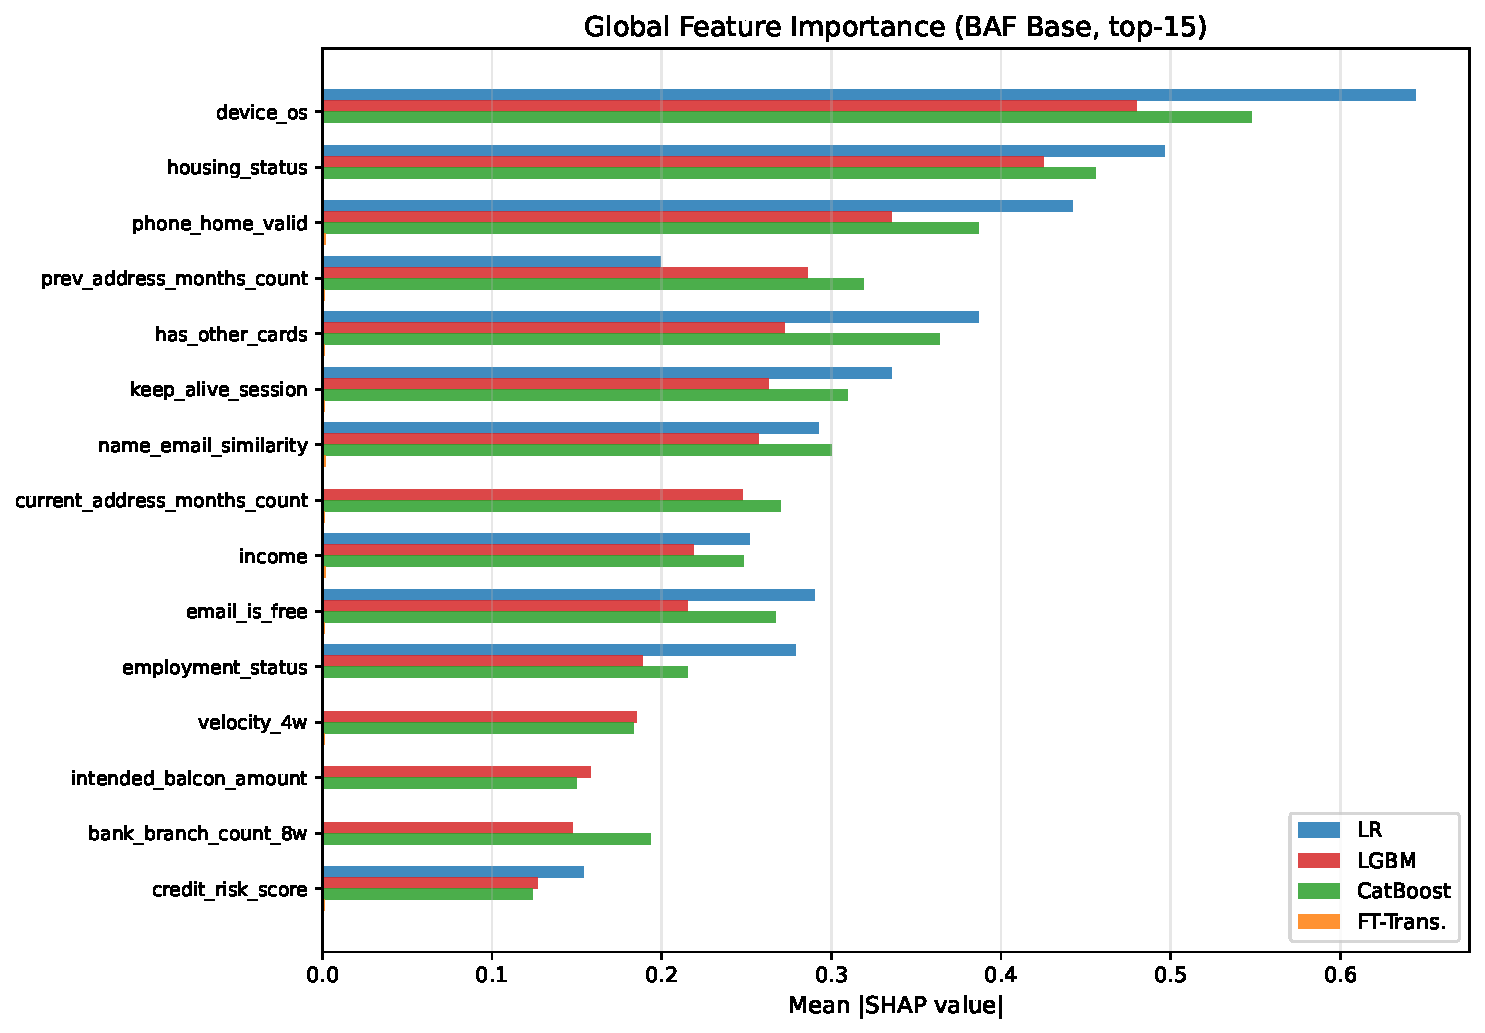
\includegraphics[width=0.88\textwidth]{figures/baf/shap_global.pdf}
  \caption{Top-15 features by mean $|\text{SHAP}|$ on BAF Base for LR, LGBM, CatBoost, and FT-Transformer.}
  \label{fig:shap_global}
\end{figure}

\begin{figure}[ht!]
  \centering
  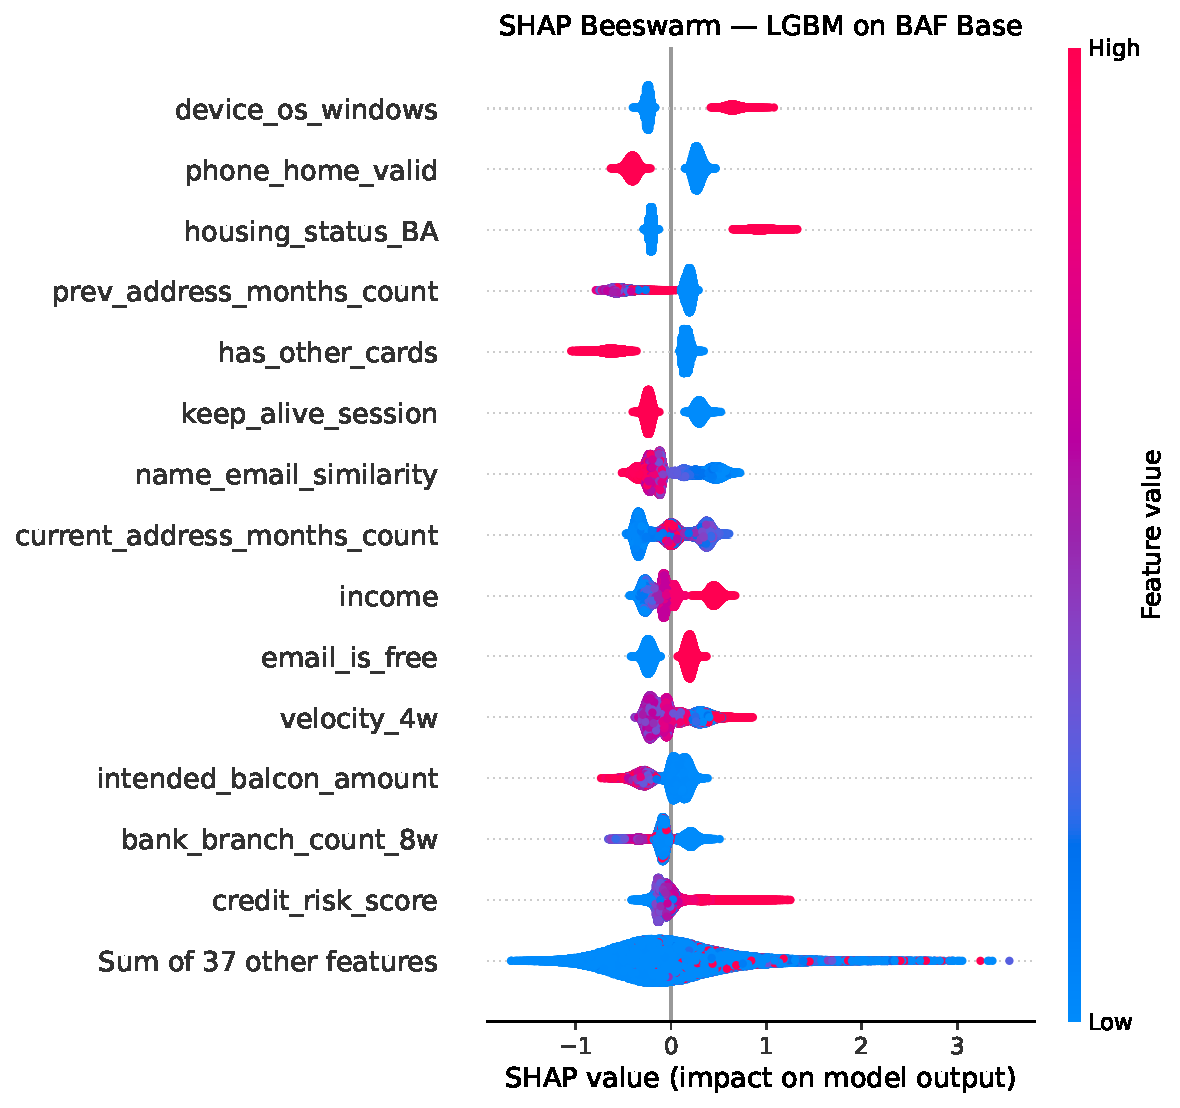
\includegraphics[width=0.88\textwidth]{figures/baf/shap_beeswarm.pdf}
  \caption{SHAP beeswarm plot for LGBM on BAF Base. Each dot represents a test sample;
    colour indicates feature value (red\,=\,high, blue\,=\,low).
    Features are sorted by mean $|\text{SHAP}|$.}
  \label{fig:shap_beeswarm}
\end{figure}

\subsection{Cross-Model Feature Consistency}

\begin{table}[ht!]
\centering
\caption{Jaccard similarity of top-10 SHAP features across model pairs (BAF Base).}
\label{tab:shap_consistency}
\begin{tabular}{l c c c c}
\toprule
          & LR & LGBM & CatBoost & FT-Trans. \\
\midrule
LR         & --- & 0.67 & 0.67 & 0.33 \\
LGBM       & 0.67 & --- & 1.00 & 0.54 \\
CatBoost   & 0.67 & 1.00 & --- & 0.54 \\
FT-Trans.  & 0.33 & 0.54 & 0.54 & --- \\
\bottomrule
\end{tabular}
\end{table}

\subsection{Cross-Variant Feature Stability}

\begin{table}[ht!]
\centering
\caption{Jaccard similarity of top-10 SHAP features for LGBM across BAF Variants.}
\label{tab:shap_stability}
\begin{tabular}{l c c c c c c}
\toprule
         & Base & Var.~I & Var.~II & Var.~III & Var.~IV & Var.~V \\
\midrule
Base       & --- & 1.00 & 1.00 & 1.00 & 1.00 & 1.00 \\
Var.~I     & 1.00 & --- & 1.00 & 1.00 & 1.00 & 1.00 \\
Var.~II    & 1.00 & 1.00 & --- & 1.00 & 1.00 & 1.00 \\
Var.~III   & 1.00 & 1.00 & 1.00 & --- & 1.00 & 1.00 \\
Var.~IV    & 1.00 & 1.00 & 1.00 & 1.00 & --- & 1.00 \\
Var.~V     & 1.00 & 1.00 & 1.00 & 1.00 & 1.00 & --- \\
\bottomrule
\end{tabular}
\end{table}

\subsection{Local Explanations}

\begin{figure}[ht!]
  \centering
  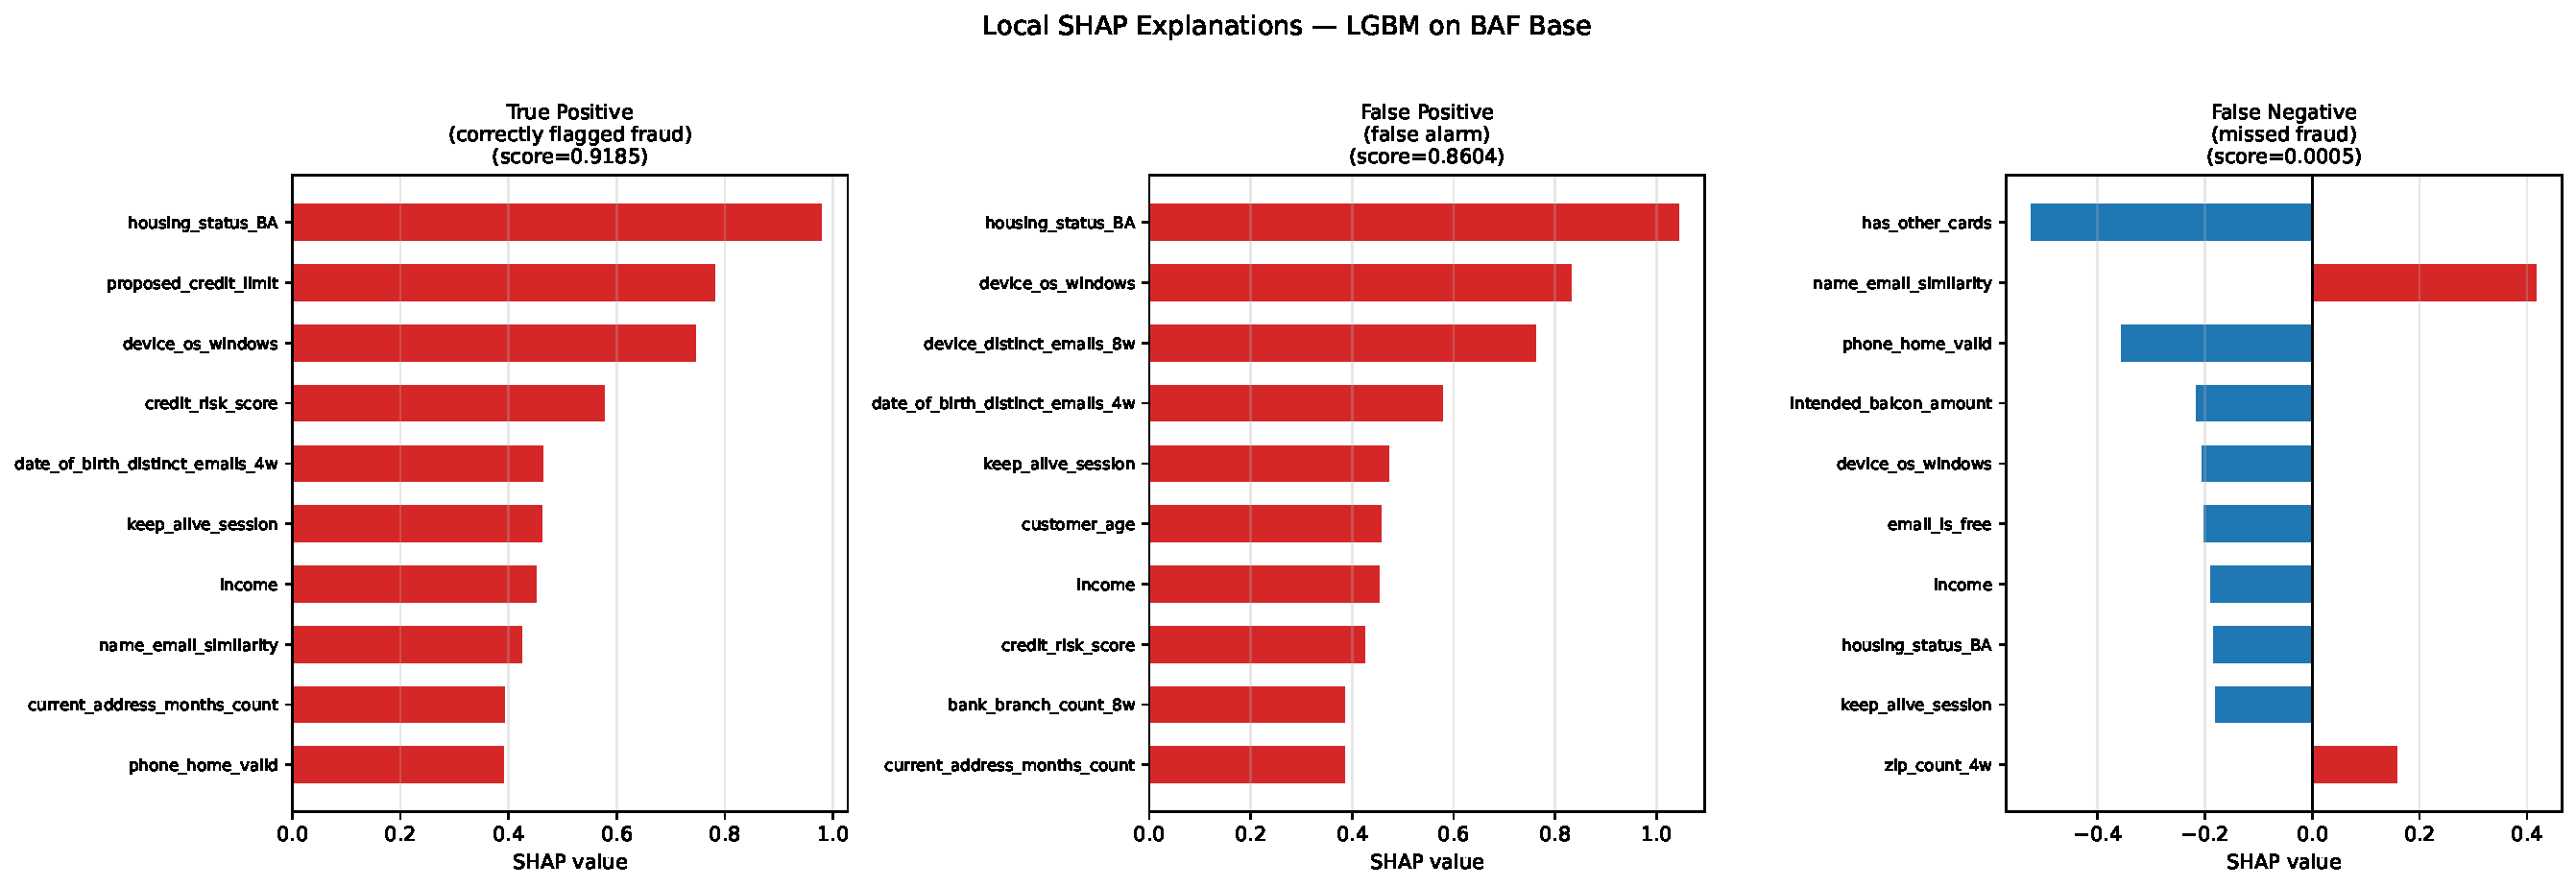
\includegraphics[width=0.95\textwidth]{figures/baf/shap_waterfall_tp_fp_fn.pdf}
  \caption{SHAP contribution plots for representative True Positive,
    False Positive, and False Negative cases (LGBM on BAF Base).
    Red bars push toward fraud; blue bars push toward legitimate.}
  \label{fig:shap_local}
\end{figure}

\subsection{Feature Dependence}

\begin{figure}[ht!]
  \centering
  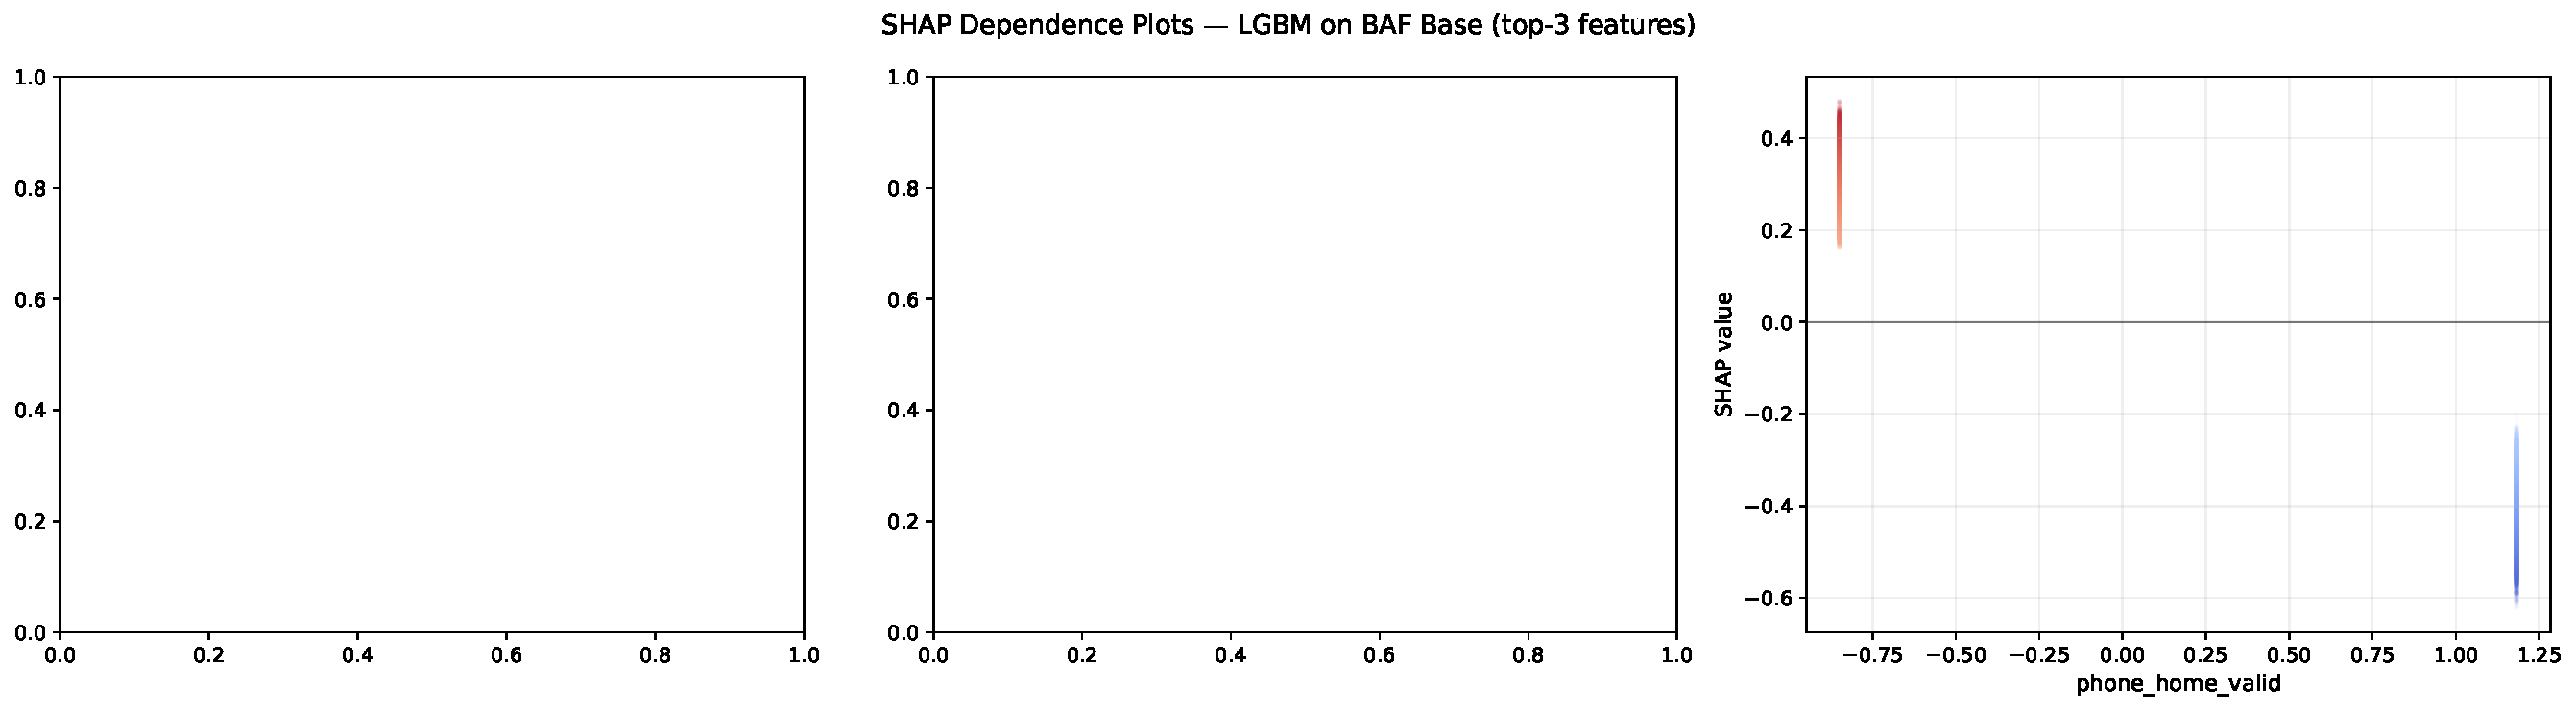
\includegraphics[width=0.95\textwidth]{figures/baf/shap_dependence.pdf}
  \caption{SHAP dependence plots for the top-3 features (LGBM on BAF Base).
    Each point is a test sample; colour intensity reflects SHAP value magnitude.}
  \label{fig:shap_dependence}
\end{figure}

\paragraph{Discussion.}
The SHAP analysis yields three key findings.

\textbf{(1)~Consistent top features across tree-based models.}
The global importance bar chart (Figure~\ref{fig:shap_global}) shows that \texttt{device\_os}, \texttt{housing\_status}, and \texttt{phone\_home\_valid} are the three most influential features for LR, LGBM, and CatBoost alike.
The cross-model consistency table (Table~\ref{tab:shap_consistency}) confirms this quantitatively: LGBM and CatBoost share an identical top-10 feature set (Jaccard\,=\,1.00), and both overlap strongly with LR (Jaccard\,=\,0.67).
This convergence across architecturally different models strengthens confidence that these features capture genuine fraud signals rather than model-specific artefacts.

\textbf{(2)~FT-Transformer learns a different feature hierarchy.}
The FT-Transformer's top features---\texttt{name\_email\_similarity}, \texttt{income}, and \texttt{phone\_home\_valid}---overlap only partially with the tree-based ranking (Jaccard\,=\,0.33--0.54 vs.\ LR/LGBM/CatBoost).
The attention mechanism appears to weight continuous features more heavily than categorical ones, which is consistent with the FT-Transformer's per-feature linear tokenisation: continuous features contribute richer gradient signals than one-hot-encoded categoricals.
This architectural divergence does not imply worse performance (the FT-Transformer matches CatBoost on PR-AUC), but it suggests that ensemble strategies combining tree-based and transformer-based models could leverage complementary feature perspectives.

\textbf{(3)~Perfect cross-variant stability.}
Table~\ref{tab:shap_stability} shows that LGBM's top-10 feature ranking is identical across all six BAF datasets (Base + Variants~I--V), yielding Jaccard\,=\,1.00 for every pairwise comparison.
This remarkable stability indicates that the features driving fraud predictions are invariant to the distributional shifts introduced by the BAF suite (covariate shift, label shift, bias conditions).
Combined with the cross-domain results (Section~\ref{sec:cross_domain_results}), this suggests that the performance degradation observed on Variants~III and~V stems from changes in the \emph{relationship} between features and the target, not from changes in feature importance ordering.

The beeswarm plot (Figure~\ref{fig:shap_beeswarm}) reveals non-linear feature effects: for instance, low values of \texttt{phone\_home\_valid} push strongly toward fraud, while \texttt{device\_os} shows a categorical split with one level dominating the fraud signal.
The local explanations (Figure~\ref{fig:shap_local}) illustrate the model's decision process for individual transactions: the True Positive case shows multiple features pushing toward fraud, whereas the False Negative is characterised by mixed signals where the legitimate-leaning features narrowly outweigh the fraud indicators.


\clearpage
% ══════════════════════════════════════════════════════════════════════════
%  7 — FT-TRANSFORMER ATTENTION DIAGNOSTICS
% ══════════════════════════════════════════════════════════════════════════

\section{FT-Transformer Attention Diagnostics}
\label{sec:attention_diagnostics}

The attention mechanism is the defining component of the FT-Transformer architecture. Analysing the learned attention weights provides a mechanistic account of how the model processes tabular features — and whether any pathological patterns explain the observed performance behaviour.

Four attention patterns are considered as candidate diagnostics for tabular transformers:
\begin{itemize}
  \item \textbf{Tunnel Vision:} one or very few features receive nearly all attention, ignoring the rest.
  \item \textbf{Self-Obsession:} the \texttt{[CLS]} classification token attends primarily to itself, blocking information flow from feature tokens.
  \item \textbf{Categorical Trap:} categorical feature tokens receive disproportionately high attention relative to numerical tokens.
  \item \textbf{Foggy Vision:} attention is near-uniformly distributed across all tokens, providing no selective emphasis on informative features.
\end{itemize}

Diagnostics were computed on 200\,000 test samples from BAF Base using the best-performing FT-Transformer configuration ($\tau = 0.058$). The model operates on 31 tokens: 25 numerical features, 5 categorical features, and the \texttt{[CLS]} classification token.

\subsection{Aggregate Attention Distribution}

\begin{figure}[ht!]
  \centering
  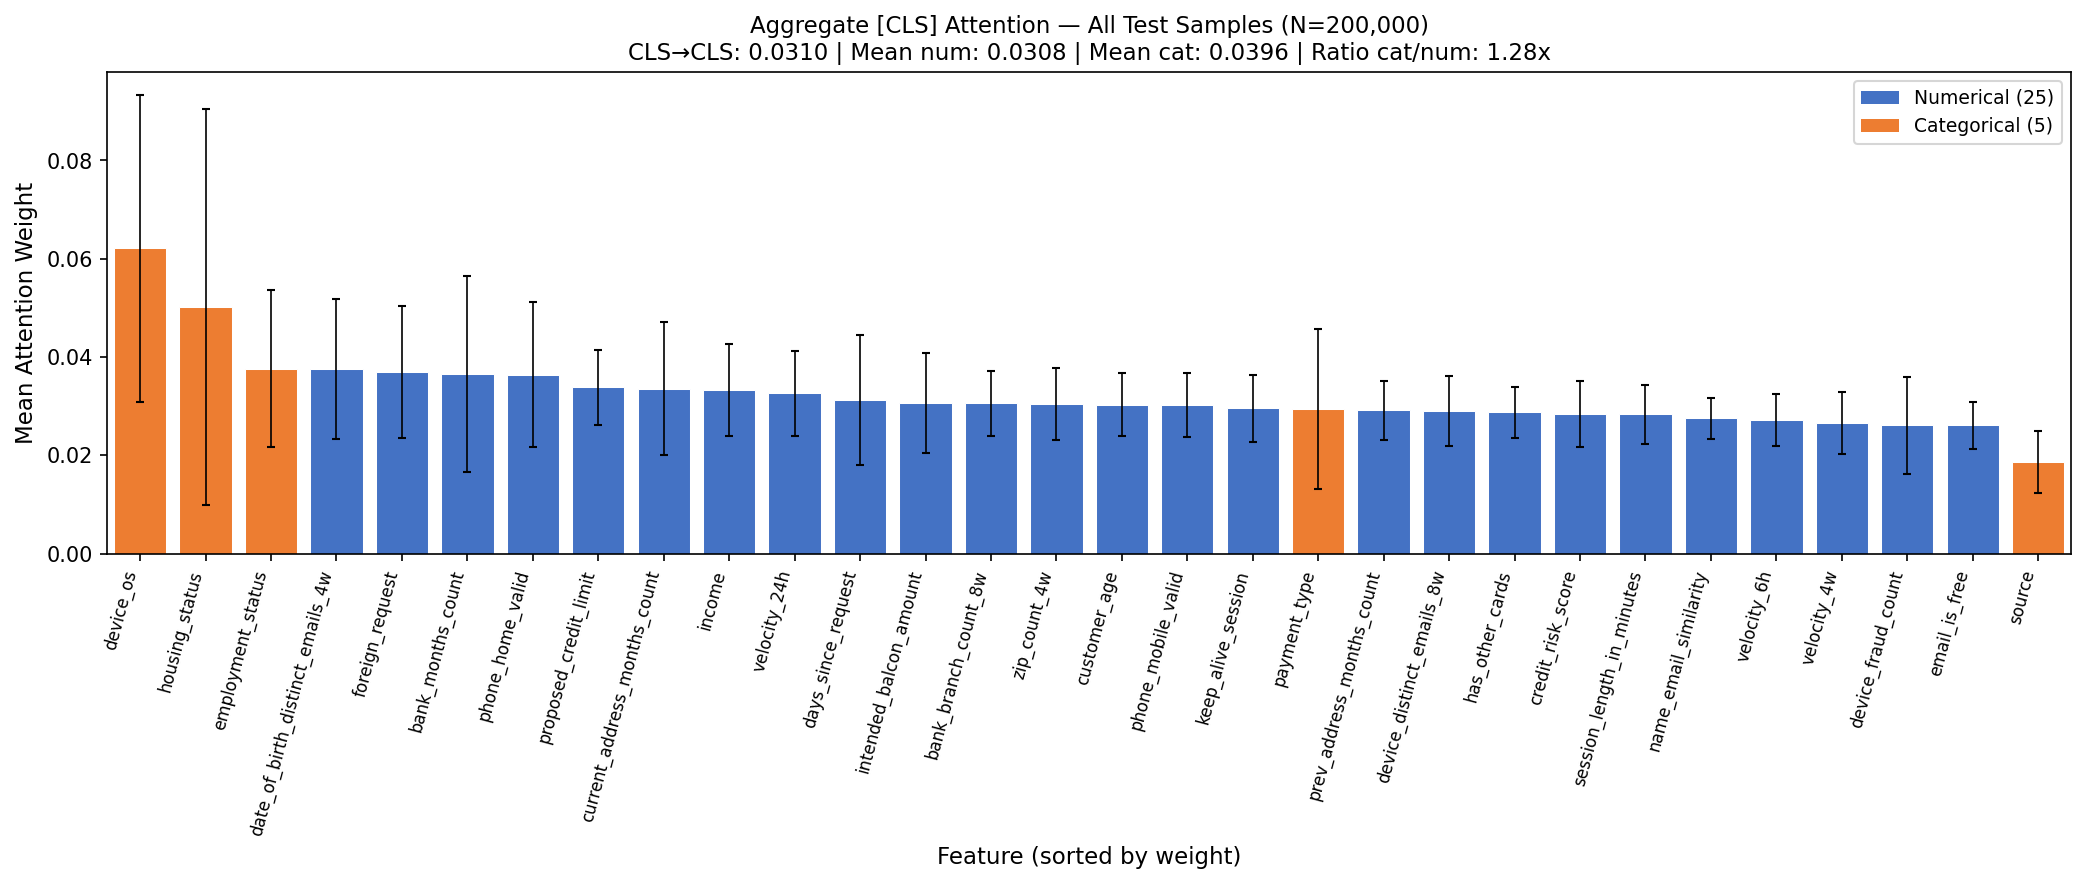
\includegraphics[width=0.95\textwidth]{figures/baf/attention_aggregate.png}
  \caption{Mean attention weight per feature token aggregated over all 200\,000 BAF Base test samples. Categorical features are shown in orange; numerical features in blue. Error bars represent standard deviation across samples. A perfectly uniform distribution would assign $1/31 \approx 3.2\%$ to each token.}
  \label{fig:attention_aggregate}
\end{figure}

Figure~\ref{fig:attention_aggregate} shows the aggregate attention distribution. The key diagnostic statistics are:

\begin{itemize}
  \item \textbf{Normalised entropy:} $H_{\text{norm}} = 0.976$. The observed entropy (3.352 nats) is 97.6\% of the theoretical maximum for 31 tokens ($\ln(31) = 3.434$ nats), confirming near-uniform attention.
  \item \textbf{\texttt{[CLS]} self-attention:} 3.1\%, indistinguishable from the uniform baseline of $1/31 \approx 3.2\%$ — ruling out Self-Obsession.
  \item \textbf{Mean categorical vs.\ numerical attention:} 4.0\% vs.\ 3.1\% (ratio 1.28$\times$) — a slight categorical elevation, far below what would constitute a Categorical Trap.
  \item \textbf{Top tokens by attention:} \texttt{device\_os} (6.2\%), \texttt{housing\_status} (5.0\%), \texttt{employment\_status} (3.8\%) — consistent with the SHAP-based feature importance reported in Section~\ref{sec:shap_results}.
\end{itemize}

\textbf{Diagnosis: Foggy Vision.} The model does not exhibit Tunnel Vision, Self-Obsession, or Categorical Trap. Attention is broadly and near-uniformly distributed across all 31 feature tokens.

\subsection{Individual Case Attention Heatmaps}

\begin{figure}[ht!]
  \centering
  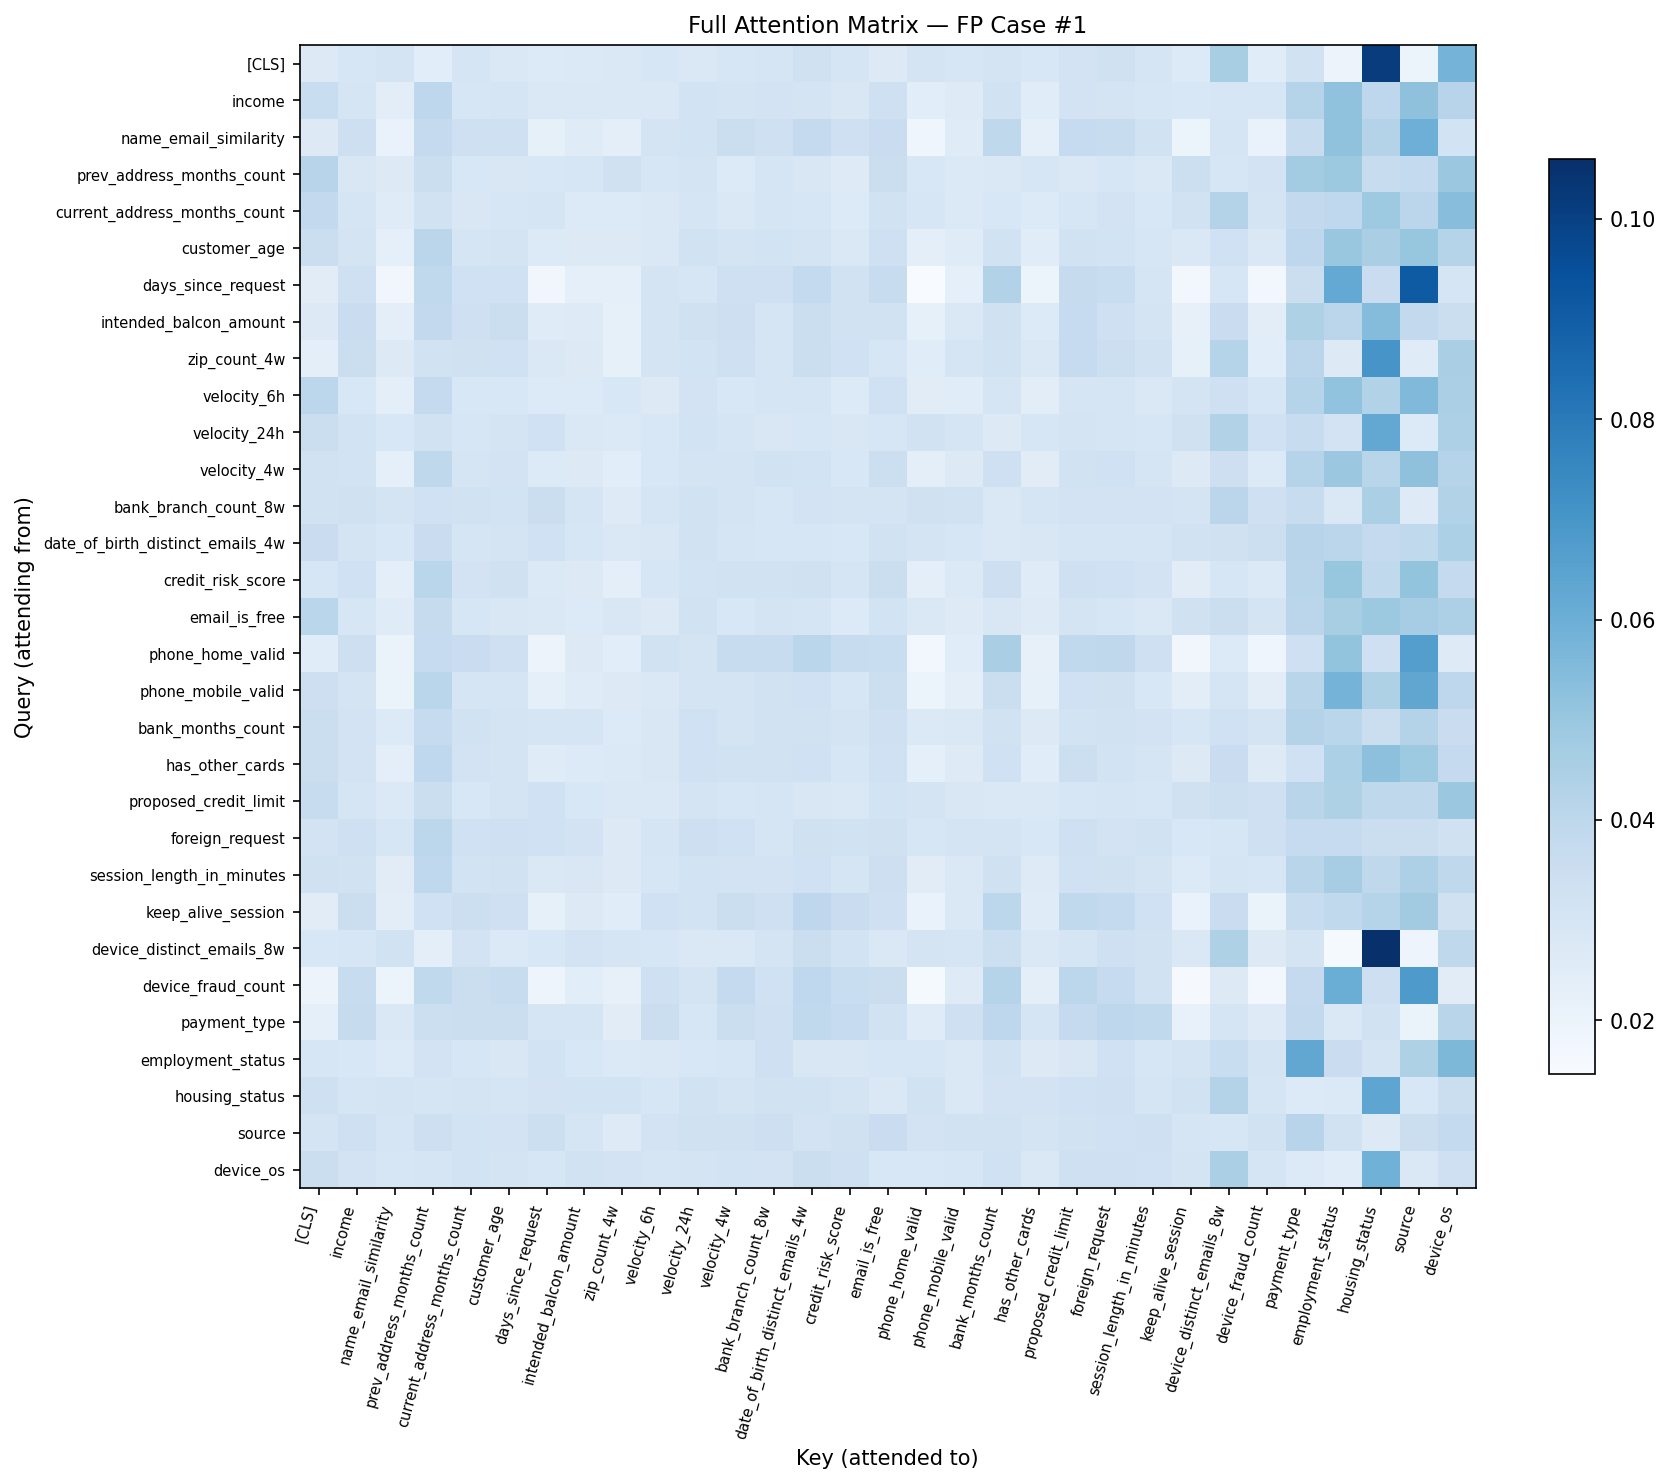
\includegraphics[width=0.80\textwidth]{figures/baf/attention_heatmap_fp.png}
  \caption{Full $31{\times}31$ attention matrix for a representative False Positive case (score\,$\approx\tau = 0.0584$). Each cell $(i,j)$ shows the attention weight from query token $i$ to key token $j$. The near-uniform light-blue colouration across the entire matrix confirms the Foggy Vision pattern at the individual case level.}
  \label{fig:attention_heatmap_fp}
\end{figure}

Figure~\ref{fig:attention_heatmap_fp} shows the full attention matrix for a borderline False Positive case (score just above threshold). The matrix is dominated by near-uniform low attention, with marginal concentration on \texttt{device\_os} and \texttt{housing\_status}. False Negative cases (scores just below threshold) exhibit the same qualitative pattern. In both cases, there is no single feature that the model focuses on — the classification emerges from a broad, distributed aggregation of all feature representations.

\paragraph{Discussion.}
The Foggy Vision diagnosis has a direct interpretive implication for the thesis's central question. The FT-Transformer is not performing at 0.18~PR-AUC because its attention mechanism is broken or degenerate: no pathological pattern is present. Rather, the model genuinely integrates information across all features, but the BAF dataset does not contain sufficient discriminative signal to reward selective attention. This is consistent with the dataset-ceiling interpretation advanced in Sections~\ref{sec:baseline_results} and~\ref{sec:cross_domain_results}: the 0.18~PR-AUC reflects a limit of the available information in the feature space, not a model-specific failure.

The slight residual categorical preference (1.28$\times$) aligns with the FT-Transformer's tokenisation design, in which categorical embeddings carry richer discrete representations than linear numeric projections, but does not translate into a performance advantage over tree-based models that handle the same categorical features natively via splitting. The perfect alignment between the top attention tokens (\texttt{device\_os}, \texttt{housing\_status}) and the top SHAP features of tree-based models indicates that the FT-Transformer has converged to the same information sources, through a different inductive pathway. Collectively, the attention diagnostics confirm that the competitive parity between FT-Transformer and CatBoost on BAF is genuine: further gains on this dataset would require richer features or additional data sources rather than architectural changes to the transformer.

\clearpage
% ══════════════════════════════════════════════════════════════════════════
%  8 — CONSOLIDATED SUMMARY
% ══════════════════════════════════════════════════════════════════════════

\section{Consolidated Summary}
\label{sec:consolidated}

\subsection{PR Curves~--- All Models Overlaid (Baseline)}

\begin{figure}[ht!]
  \centering
  
\includegraphics[width=0.48\textwidth]{figures/ulb/pr_curves_baseline.pdf}%
  \hfill
  
\includegraphics[width=0.48\textwidth]{figures/baf/pr_curves_baseline.pdf}
  \caption{Precision--Recall curves for all models on ULB~2013 (left) and BAF~Base (right) under the baseline setting (strategy\,=\,None). OCSVM is included for reference.}
  \label{fig:pr_curves_consolidated}
\end{figure}

The PR curves visually confirm the quantitative findings from the baseline tables. On ULB~2013, CatBoost, LGBM, RF, and FT-Transformer produce curves that dominate the upper-right region, while LR is slightly lower and OCSVM collapses near the origin. On BAF~Base, all curves are compressed into the low-precision region, reflecting the inherent difficulty of the dataset; the supervised models are tightly clustered, with OCSVM again clearly separated.

\subsection{Decision Framework}

\begin{table}[ht!]
\centering
\caption{Decision framework: recommended configuration by deployment scenario. Recommendations are derived from the experimental results presented in Sections~\ref{sec:baseline_results}--\ref{sec:shap_results}.}
\label{tab:decision_framework}
\begin{tabular}{p{4.2cm} l l l}
\toprule
Scenario & Model & Strategy & Threshold \\
\midrule
High recall, ULB-like      & CatBoost  & None / ROS   & max-$F_2$      \\
Balanced $F_1$, ULB-like   & CatBoost  & None         & max-$F_1$      \\
High recall, BAF-like      & LGBM      & None / Weights & max-$F_2$    \\
Balanced $F_1$, BAF-like   & CatBoost  & ROS          & max-$F_1$      \\
Cross-domain deployment    & RF        & None         & max-$F_2$      \\
Interpretability required  & LGBM      & None         & max-$F_2$      \\
Low workload budget        & CatBoost  & None         & Prec$\geq$0.5  \\
\bottomrule
\end{tabular}
\end{table}

The decision framework synthesises the experimental evidence into actionable recommendations.
CatBoost is the default choice for in-domain deployment due to its consistently top-tier performance on both datasets.
For cross-domain scenarios where distribution shift is expected, Random Forest is preferred despite lower in-domain scores, given its superior robustness (Section~\ref{sec:cross_domain_results}).
When interpretability is a requirement, LGBM offers the best balance of performance and SHAP-based explainability (Section~\ref{sec:shap_results}), as its feature importance ranking is identical to CatBoost's (Jaccard\,=\,1.00) while being computationally lighter.
The Precision$\geq$0.5 threshold is recommended when investigation capacity is limited, accepting lower recall to ensure that at least half of all alerts are genuine fraud.

\subsection{Bootstrap Confidence Intervals}

\begin{table}[ht!]
\centering
\caption{95\% Bootstrap CI for PR-AUC and ROC-AUC on ULB 2013 (strategy\,=\,None, 1\,000 iterations).}
\label{tab:ci_ulb}
\begin{tabular}{l c c c c}
\toprule
Model & PR-AUC & 95\% CI & ROC-AUC & 95\% CI \\
\midrule
LR         & 0.742 & [0.653, 0.823] & 0.965 & [0.943, 0.985] \\
RF         & 0.867 & [0.796, 0.927] & 0.959 & [0.930, 0.986] \\
LGBM       & 0.874 & [0.811, 0.929] & 0.975 & [0.955, 0.994] \\
CatBoost   & 0.885 & [0.824, 0.940] & 0.978 & [0.957, 0.995] \\
FT-Trans.  & 0.856 & [0.791, 0.914] & 0.975 & [0.951, 0.996] \\
OCSVM      & 0.335 & [0.252, 0.449] & 0.953 & [0.922, 0.979] \\
\bottomrule
\end{tabular}
\end{table}

\begin{table}[ht!]
\centering
\caption{95\% Bootstrap CI for PR-AUC and ROC-AUC on BAF Base (strategy\,=\,None, 1\,000 iterations).}
\label{tab:ci_baf}
\begin{tabular}{l c c c c}
\toprule
Model & PR-AUC & 95\% CI & ROC-AUC & 95\% CI \\
\midrule
LR         & 0.143 & [0.131, 0.158] & 0.875 & [0.867, 0.882] \\
RF         & 0.159 & [0.145, 0.175] & 0.878 & [0.870, 0.885] \\
LGBM       & 0.177 & [0.162, 0.194] & 0.898 & [0.892, 0.905] \\
CatBoost   & 0.180 & [0.164, 0.197] & 0.898 & [0.892, 0.904] \\
FT-Trans.  & 0.180 & [0.164, 0.197] & 0.897 & [0.891, 0.904] \\
OCSVM      & 0.019 & [0.018, 0.021] & 0.628 & [0.616, 0.639] \\
\bottomrule
\end{tabular}
\end{table}

\subsection{Computational Cost}

\begin{table}[ht!]
\centering
\caption{Computational cost on ULB 2013 (strategy\,=\,None). Tuning includes Optuna TPE (50 trials, 5-fold CV).}
\label{tab:cost_ulb}
\begin{tabular}{l r r r}
\toprule
Model & Tuning (s) & Train (s) & Inference (s) \\
\midrule
LR         & 30,491 & 242.1 & 0.104 \\
RF         & 94,977 & 609.9 & 1.671 \\
LGBM       & 305 & 1.8 & 0.135 \\
CatBoost   & 7,456 & 41.5 & 0.131 \\
FT-Trans.  & 15,598 & 262.9 & 1.074 \\
OCSVM      & --- & 98.1 & 10.117 \\
\bottomrule
\end{tabular}
\end{table}

\begin{table}[ht!]
\centering
\caption{Computational cost on BAF Base (strategy\,=\,None). Tuning includes Optuna TPE (50 trials, 5-fold CV).}
\label{tab:cost_baf}
\begin{tabular}{l r r r}
\toprule
Model & Tuning (s) & Train (s) & Inference (s) \\
\midrule
LR         & 55,070 & 83.9 & 0.321 \\
RF         & 105,313 & 1494.0 & 21.075 \\
LGBM       & 1,243 & 16.1 & 1.387 \\
CatBoost   & 7,010 & 36.7 & 0.249 \\
FT-Trans.  & 46,550 & 346.9 & 2.419 \\
OCSVM      & --- & 919.6 & 71.579 \\
\bottomrule
\end{tabular}
\end{table}


\clearpage
% ══════════════════════════════════════════════════════════════════════════
% DISCUSSION
% ══════════════════════════════════════════════════════════════════════════

\section{Discussion}
\label{sec:discussion}

\subsection{Classical ML vs.\ Transformer for Fraud Detection}

The FT-Transformer achieves competitive but not superior performance relative to gradient-boosted trees.
On ULB~2013, it reaches PR-AUC\,=\,0.856, placing it between RF~(0.867) and LR~(0.742) but below CatBoost~(0.885) and LGBM~(0.873).
On the larger BAF~Base ($N$\,=\,1M), the FT-Transformer matches CatBoost exactly (PR-AUC\,=\,0.180), suggesting that attention-based models benefit from increased data volume---consistent with the general observation that deep learning methods require more training examples to reach their potential.

However, the FT-Transformer is less robust to imbalance handling strategies than tree-based models (Section~\ref{sec:transformer_imbalance}): SMOTE degrades its PR-AUC by 41\% on BAF, compared to only 14\% for CatBoost.
The Class Weights strategy (modifying the loss function) is the safest imbalance intervention for the FT-Transformer, preserving baseline performance on both datasets.

From a practical standpoint, the FT-Transformer's training cost is substantially higher---requiring GPU computation, epoch-based optimisation with early stopping, and careful hyperparameter tuning---while offering no performance advantage over CatBoost or LGBM on these datasets.
Its primary value lies in providing a complementary feature perspective (Section~\ref{sec:shap_results}), which could be leveraged in ensemble strategies.

\subsection{Threshold Selection Matters}

The threshold sensitivity analysis reveals one of the most practically significant findings of this thesis.
On ULB~2013, where fraud prevalence is extremely low (0.17\%) but models produce well-separated scores, threshold choice has a moderate effect: the gap between worst and best strategy is $\sim$0.15~$F_2$ for Logistic Regression but $<$0.04 for CatBoost.
On BAF~Base ($\approx$1.1\% fraud), the effect is an order of magnitude larger: using $\tau=0.5$ reduces $F_2$ to near zero for all models, while max-$F_2$ recovers values in the 0.29--0.32 range.

This asymmetry has a clear explanation.
ULB models, tuned on a dataset where the positive class is extremely rare, learn to output high confidence scores for true positives; thus, most fraud cases already exceed~0.5.
BAF models, facing a less extreme imbalance ratio but more complex feature interactions, produce lower and more spread-out probability scores; the optimal threshold lies in the 0.05--0.10 range, far from the default.

From a practical standpoint, these results confirm that \textbf{any deployment of a fraud detection system must include an explicit threshold calibration step}.
Using a fixed 0.5 threshold---the default in most ML frameworks---is acceptable only when the positive class is already well-separated in score space, which cannot be assumed in general.

\subsection{Imbalance Strategy \texorpdfstring{$\times$}{x} Model Interaction}

The full factorial analysis yields a nuanced picture: no single imbalance strategy uniformly improves all models on both datasets.
On ULB~2013, RUS degrades every model---discarding majority-class samples from an already small dataset removes decision-boundary information.
ROS and Class Weights are neutral-to-positive for tree-based models, while SMOTE-based strategies offer marginal gains at best.
On BAF~Base, the picture is starker: no strategy improves CatBoost or LGBM beyond their baselines by more than 0.01~PR-AUC, confirming that modern gradient-boosted trees with Optuna-tuned hyperparameters handle moderate imbalance ($\approx$1.1\% positive rate) effectively without explicit resampling.

The interaction between model and strategy is the key finding.
SMOTE and SMOTE+Tomek consistently produce identical results (the Tomek cleaning removes zero borderline examples under extreme imbalance), and both degrade tree-based models on BAF while offering no benefit on ULB.
Class Weights is the most consistently safe strategy across all model families: it never degrades performance substantially and occasionally improves it (e.g., LR on ULB).
These results support the practical recommendation that practitioners should default to no resampling or class weighting for gradient-boosted models and reserve SMOTE-based strategies for specific scenarios where they have been validated on the target data.

\subsection{Cross-Domain Generalization}

The cross-domain experiment confirms that model robustness under distribution shift does not follow the same ranking as in-domain performance.
LGBM and CatBoost---the strongest models on BAF Base---suffer PR-AUC losses of 24--31\% on Variants~III and~V, which combine covariate shift with feature-space changes.
In contrast, Random Forest is the most transfer-resilient model, \emph{improving} on four out of five variants (I, II, III, and IV) and remaining stable on Variant~V.
This finding has practical implications: in deployment scenarios where the data distribution may drift over time, an ensemble strategy or periodic recalibration may be preferable to relying on a single high-performing model.

Variant~II (label shift only) is the easiest transfer target for all models, confirming that changes in fraud prevalence alone do not degrade discriminative performance when feature distributions remain stable.

ULB~$\leftrightarrow$~BAF cross-dataset transfer is not feasible due
to incompatible feature spaces (PCA-anonymised vs.\ real-world features).
This limitation is acknowledged; the BAF internal transfer setting
provides a controlled environment to study generalization with matched features.

\subsection{Performance--Interpretability Trade-offs}

The SHAP analysis demonstrates that interpretability need not come at the cost of performance.
LGBM and CatBoost---the top-performing models---produce identical feature importance rankings (Jaccard\,=\,1.00), and both are amenable to fast, exact SHAP computation via TreeExplainer.
The FT-Transformer, while competitive in predictive accuracy, relies on GradientExplainer for SHAP values, which is slower and produces a different feature ranking (Jaccard\,=\,0.54 vs.\ tree-based models).

The perfect cross-variant stability of SHAP rankings (Jaccard\,=\,1.00 across all BAF variants) is a particularly strong finding: it means that explanations generated on one dataset version remain valid under distribution shift, reducing the need for re-explanation when deploying to new domains.
This stability, combined with the local explanation capability (waterfall plots), makes tree-based SHAP a practical tool for fraud investigation teams who need to justify automated decisions.

\subsection{Threats to Validity}
\begin{itemize}
  \item \textbf{Internal:} Hyperparameter tuning budget is finite
    (50 Optuna trials per model); single holdout split rather
    than repeated random sub-sampling; reliance on two dataset families.
  \item \textbf{External:} ULB features are PCA-anonymised, limiting
    interpretability and real-world applicability of ULB-specific findings.
    BAF is synthetically generated, so fraud patterns may not fully
    reflect real-world complexity.
  \item \textbf{Construct:} PR-AUC is sensitive to the class prior;
    comparisons of absolute PR-AUC values across datasets with different
    fraud rates should be made with caution.
  \item \textbf{Statistical:} Bootstrap CIs assume the holdout test set
    is representative; with extreme imbalance, bootstrap samples may
    have very few positive examples, widening CIs.
\end{itemize}
